\begin{frame}[noframenumbering, plain]{Overview of results}
 
\vspace{-0.4em}
\begin{center}
\resizebox{\textwidth}{!}{%
\begin{tikzpicture}[
    chip/.style={rounded corners=3pt, draw=black!30, fill=white, align=center,
               font=\tiny, inner sep=5pt, text width=4.7cm},
    hdr/.style={font=\small\bfseries, align=center, text width=5.0cm}
]
 
% --- the two banners ----------------------------------------------------------
\fill[phasecol, fill opacity=0.16, rounded corners=16pt] (-6.6,-2.7) rectangle (-0.2,2.5);
\fill[gaugecol, fill opacity=0.16, rounded corners=16pt] ( 0.2,-2.7) rectangle ( 6.6,2.5);
\draw[phasecol!55, rounded corners=16pt] (-6.6,-2.7) rectangle (-0.2,2.5);
\draw[gaugecol!55, rounded corners=16pt] ( 0.2,-2.7) rectangle ( 6.6,2.5);
 
\node[hdr, text=phasecol!80!black] at (-3.4,1.95) {Quantum phases\\[-2pt] of matter};
\node[hdr, text=gaugecol!80!black] at ( 3.4,1.95) {Gauging, dualities\\[-2pt] and anomalies};
 
% --- phases of matter ---------------------------------------------------------
\node[chip] at (-3.4, 0.7)
  {\textbf{Mapping between Morita-equivalent string-net states with a constant depth quantum circuit}\\[2pt]
   \color{black!55}PRB \textbf{105}, 085130 (2022)};
\node[chip] at (-3.4, -1.25)
  {\textbf{One-dimensional symmetric phases protected by frieze symmetries}\\[2pt]
   \color{black!55}PRB \textbf{107}, 115123 (2023)};
 
% --- gauging ------------------------------------------------------------------
\node[chip] at (3.4, 1.00)
  {\textbf{From gauging to duality in one-dimensional quantum lattice models}\\[2pt]
   \color{black!55}SciPost Phys.\ \textbf{20}, 113 (2026)};
\node[chip] at (3.4,-0.35)
  {\textbf{Twisted gauging and topological sectors in (2+1)d abelian lattice gauge theories}\\[2pt]
   \color{black!55}SciPost Phys.\ \textbf{19}, 054 (2025)};
\node[chip] at (3.4,-1.70)
  {\textbf{Systematic construction of stabilizer codes via gauging abelian boundary symmetries}\\[2pt]
   \color{black!55}Quantum \textbf{9}, 1852 (2025)};
 
% --- the common toolbox -------------------------------------------------------
\fill[toolcol, fill opacity=0.13, rounded corners=10pt] (-6.6,-3.85) rectangle (6.6,-2.85);
\node[align=center, font=\scriptsize, text=black!70, text width=12.6cm] at (0,-3.35)
    {\textbf{Les Houches Lecture Notes on Tensor Networks}\\[2pt]
   \color{black!55}SciPost Phys.\ Lect.\ Notes \textbf{128} (2026)};
 
\end{tikzpicture}}
\end{center}


\end{frame}

\begin{frame}[noframenumbering, plain]{Experimental realisations}
    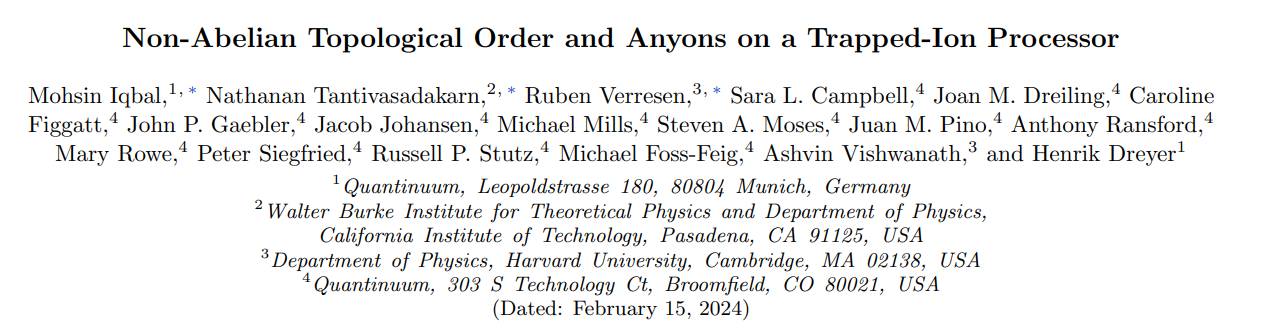
\includegraphics[width=.69\textwidth]{figs/NonAbelianTO_header.png}
    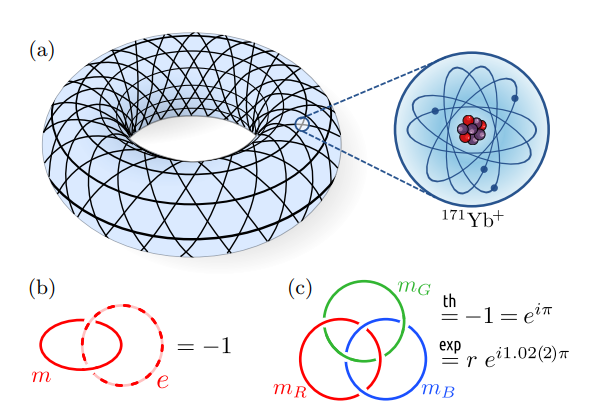
\includegraphics[width=.30\textwidth]{figs/NonAbelianTO_fig.png}

    \centering
    Realisation $\mathcal Z({\rm Vec}_{\mathbb Z_2^{3}}^\alpha)\simeq \mathcal Z({\rm Vec}_{D_4})$.
\end{frame}
\begin{frame}[noframenumbering, plain]{Experimental realisations}
\centering
    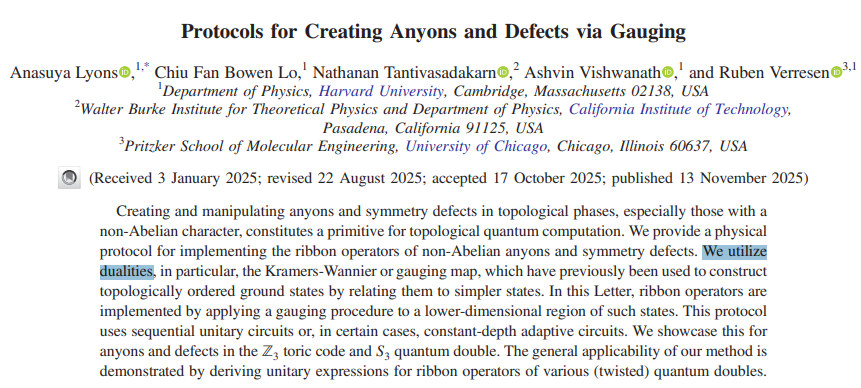
\includegraphics[width=.69\textwidth]{figs/NonAbelianTO_ribbon.png}
\end{frame}


\begin{frame}[noframenumbering, plain]{Reception}
\begin{columns}[c]
\column{.52\textwidth}
\centering
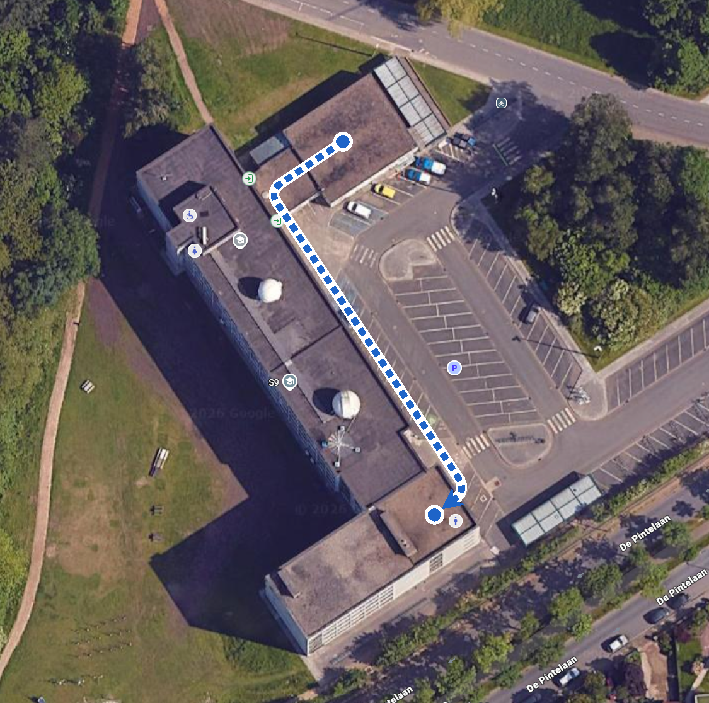
\includegraphics[width=\textwidth]{figs/MMZ_to_A1.pdf}
\column{.44\textwidth}
\centering
Parked on campus?

\smallskip
You (may) need a \emph{day ticket} to leave.

\bigskip
{\color{gray}Geparkeerd op de campus?

\smallskip
Je hebt (misschien) een \emph{dagticket} nodig om te vertrekken.}
\end{columns}
\end{frame}

\begin{frame}[noframenumbering, plain]{Image credits}
\centering
\footnotesize
\begin{tabular}{ll}
Water drop & J.~M.~Su\'arez (CC BY 2.0) \\
Ice & S.~Mollerus (CC BY 2.0) \\
Diamond & G.~Parent \\
Calcite & Danpl \\
Calcite structure & after Dove et al., Phys.\ Chem.\ Miner.\ (2005) \\
Space groups & F.~Hoffmann (CC BY-NC-SA) \\
% Honeycomb & ? \\
% Mosaic & ? \\
Curie, Landau & Wikipedia \\
% Water waves & ? \\
Experiments & Iqbal et al., Nature (2024); Lyons et al., PRL (2025)
\end{tabular}
\end{frame}